% !TEX program = xelatex
\documentclass[compress, 10pt, aspectratio=169]{beamer}

% XeLaTeX fonts
\usepackage{fontspec}

\usepackage{appendixnumberbeamer}

\usetheme[progressbar=frametitle, numbering=fraction]{metropolis}
\useoutertheme[footline=empty, subsection=false]{miniframes}
\setbeamercolor{section in head/foot}{fg=white, bg=mDarkTeal}
\setbeamertemplate{section in toc}[sections numbered]
%\setbeamertemplate{bibliography item}{\insertbiblabel}

\author{Marlene Heinrich\and Gregor Suchan}
\title{\LaTeX{}-Anfängerkurs}
\date{03.~Juli 2022}
\institute{Albert-Ludwigs-Universität Freiburg}

% Babel
\usepackage[ngerman]{babel}

% Pretty tables
\usepackage{booktabs}

% Typesetting
\usepackage{amsmath,amssymb,dsfont,mathtools,amsthm}

% Code listings
\usepackage{csquotes}

% siunitx because its good
\usepackage[locale=DE, separate-uncertainty=true]{siunitx}

% Citations
\usepackage[date=year, isbn=false, doi=false, url=false, eprint=false]{biblatex}
\addbibresource{references.bib}

\usepackage{graphicx}

\usepackage{tikz}

% Only for advanced humorous purposes.
\usepackage{soul}


\begin{document}

\begin{frame}[plain]
  \titlepage
\end{frame}

{
  \setbeamertemplate{headline}{}
  \addtobeamertemplate{frametitle}{\vspace*{-\headheight}}{}
}

\begin{frame}[plain]
  \tableofcontents
\end{frame}

\section{Das Drumherum}
\begin{frame}[plain]{Worüber reden wir eigentlich?}
  \begin{itemize}
    \item[\bfseries\TeX:]
      Textsatzsystem als Makrosprache
      \begin{itemize}
        \item
          1978 von Donald Knuth entwickelt
        \item
          Extrem feine Kontrolle über Textsatz
      \end{itemize}
    \item[\bfseries\LaTeX:]
      Sehr große Makrosammlung für \TeX{}
      \begin{itemize}
        \item
          1984 von Leslie Lamport geschrieben
        \item
          An \TeX{} angelehnter Syntax
        \item
          Fokus beim Schreiben liegt dann beim Inhalt des Dokuments
        \item
          \LaTeX{} übernimmt das Schriftsetzen
      \end{itemize}
  \end{itemize}
\end{frame}

\begin{frame}{Der Schreibvorgang}
	\begin{itemize}
	  \item
      Das Dokument wird in eine \texttt{.tex}-Datei geschrieben und dann
      kompiliert, meistens in eine \texttt{.pdf}-Datei
    \item
      Anders als bei anderen Testsatzsystemen ist das Geschriebene nicht das,
      was man sofort sieht: \LaTeX{} ist nicht WYSIWYG (What You See Is What
      You Get)
	\end{itemize}
\end{frame}

\begin{frame}{\LaTeX{}-Maschinen}
  Um die ganzen witzigen Befehle wie \texttt{pdflatex}, \texttt{latexmk} und so
  nutzen zu können, müssen diese installiert werden.
  \begin{center}
    \begin{tabular}{cc}
      \toprule
      Plattform & Pakete \\
      \midrule
      Windows, OS X & \texttt{MiKTeX} \\
      Linux-Zeug & \texttt{texlive} \\
      \bottomrule
    \end{tabular}
  \end{center}
\end{frame}

\begin{frame}{\LaTeX{}-Editoren}
  \begin{itemize}
    \item
      Da man nur in eine \texttt{.tex}-Datei schreibt, kann man dafür
      eigentlich einen gewöhnlichen Texteditor benutzen
    \item
      Da man aber an dem Geschriebenen orientieren will, sind viele
      \LaTeX-Editoren in \texttt{.tex}- und \texttt{.pdf}-Datei aufgeteilt
  \end{itemize}

\end{frame}

\begin{frame}
  \begin{center}
    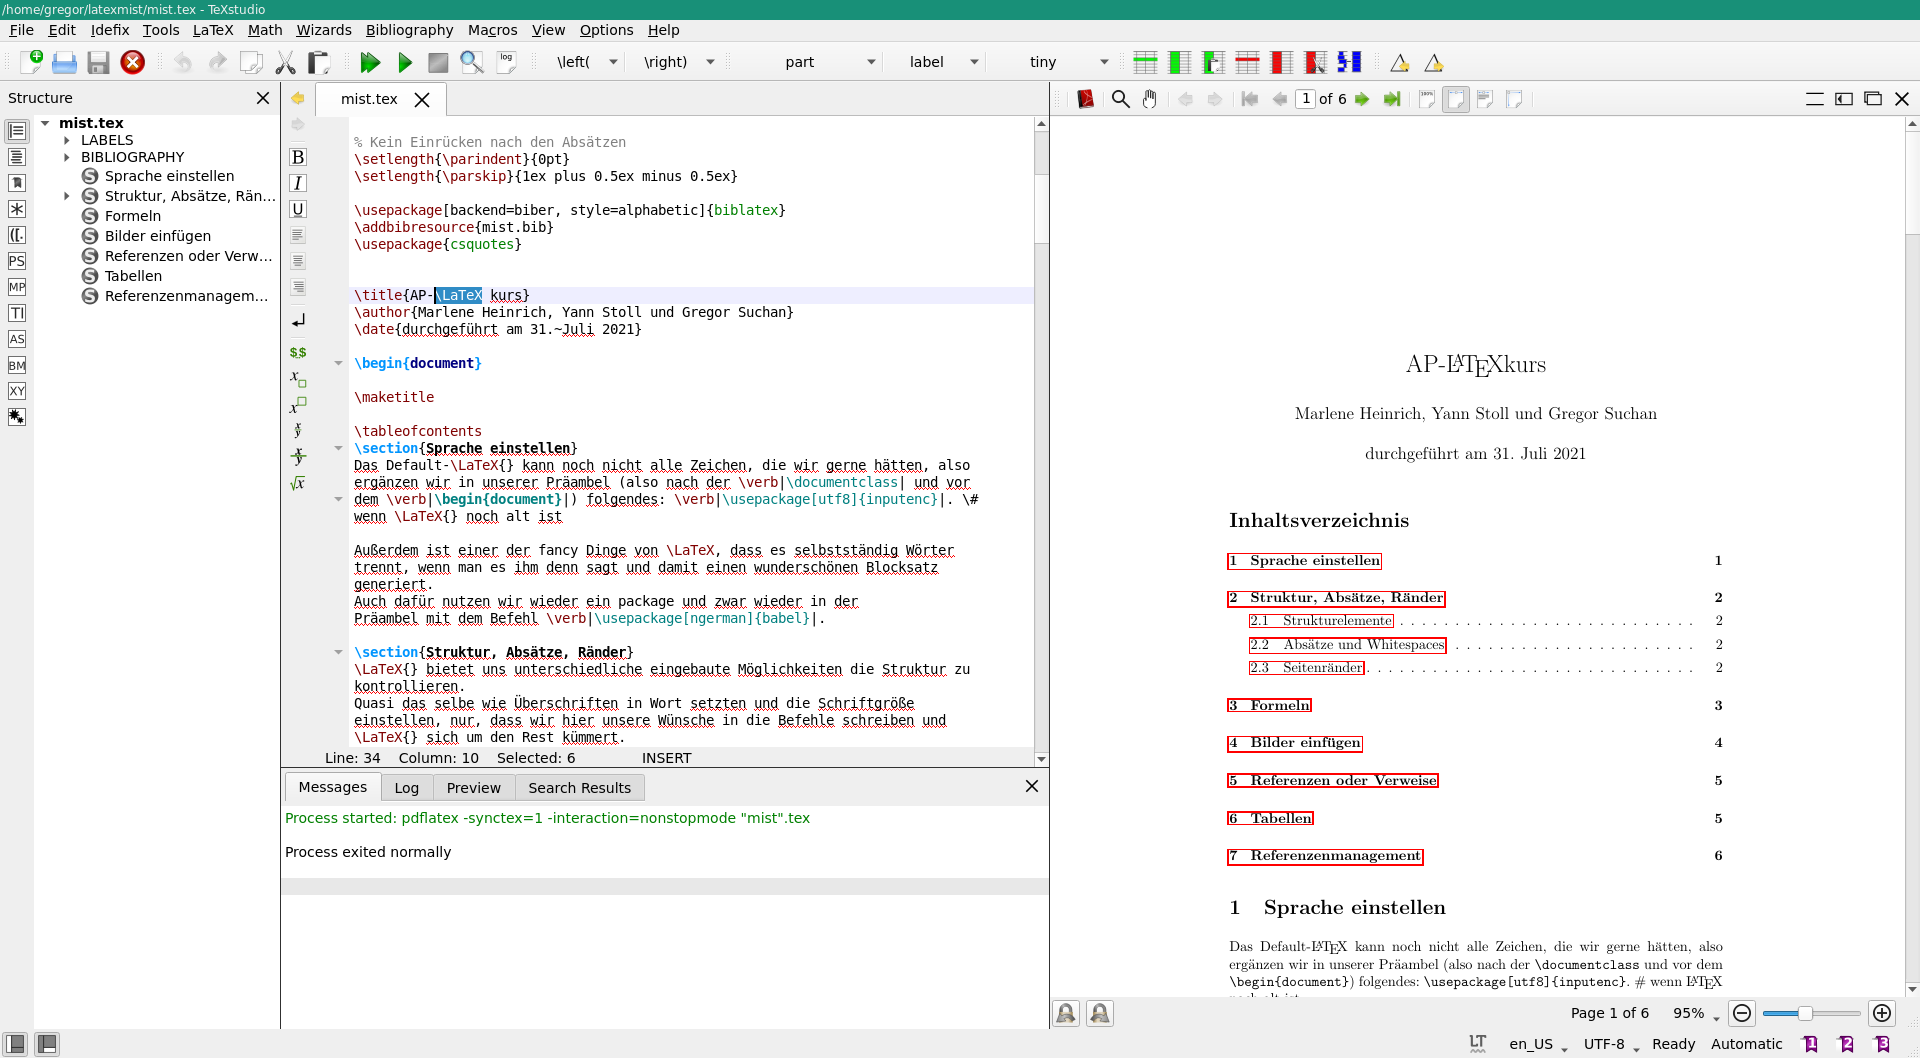
\includegraphics[width=.9\textwidth]{./texstudio.png}
  \end{center}
\end{frame}

\begin{frame}
  \begin{center}
    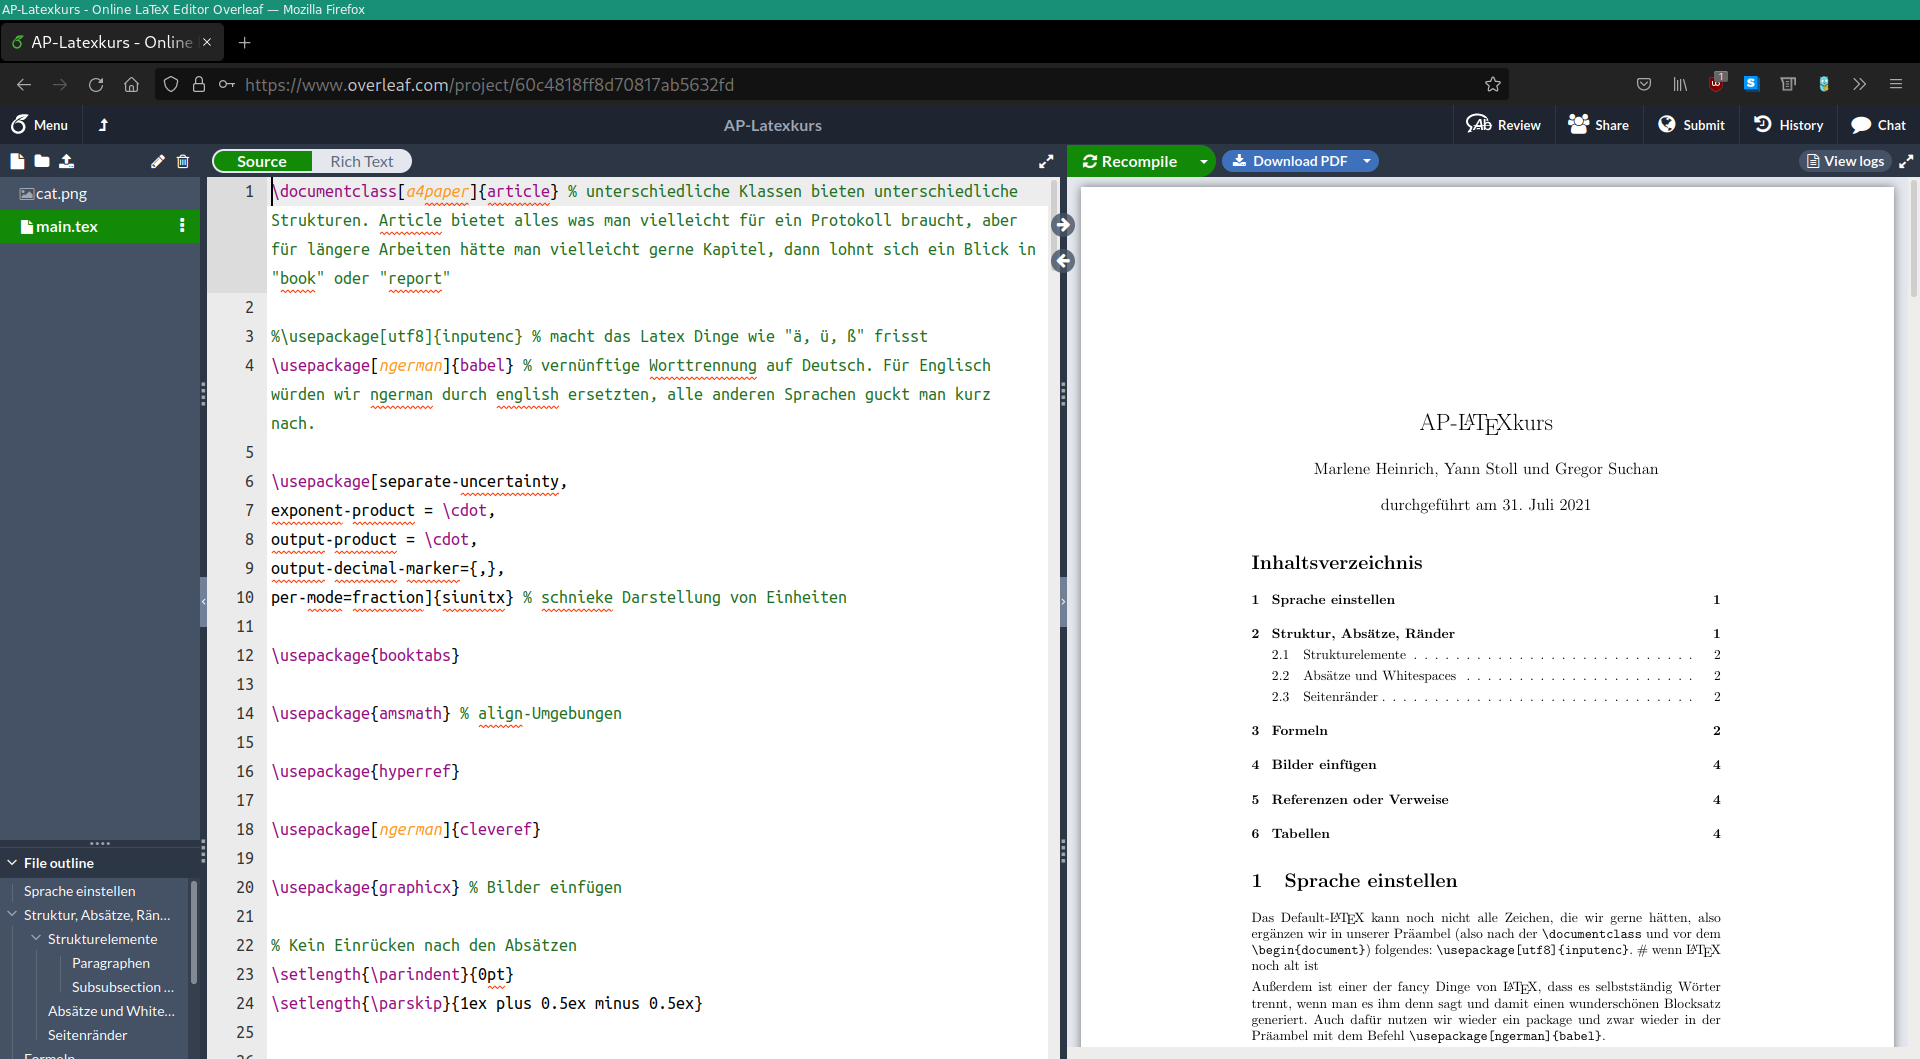
\includegraphics[width=.9\textwidth]{./overleaf.png}
  \end{center}
\end{frame}

\begin{frame}{Das Bedienen von \LaTeX{}-Editoren}
  One-shot compilation:
  \begin{center}
    \begin{tikzpicture}
      \node
        at (-4, 1)
        {\textbf{Linke Seite}};
      \node
        at (4, 1)
        {\textbf{Rechte Seite}};
      \node[draw, rectangle]
        (dat)
        at (-4, 0)
        {\texttt{.tex}-Datei};
      \node[draw, rectangle]
        (pdf)
        at (4, 0)
        {\texttt{.pdf}-Datei};
      \draw[thick, ->] (dat) -- (pdf)
        node[midway, fill=white]
        {Grüner Knopf};
    \end{tikzpicture}
  \end{center}
  Continuous compilation:
  \begin{itemize}
    \item Das Programm hält nach Änderungen in der \texttt{.tex}-Datei Ausschau
      und kompiliert automatisch neu, falls die \texttt{.tex} gespeichert wurde
      und jetzt anders ist.
  \end{itemize}
\end{frame}

\section{Das Wesentliche}

\begin{frame}[fragile]{Struktur der \texttt{.tex}-Datei}
  Folgende Dinge sind für \LaTeX{} obligatorisch:
  \begin{itemize}
    \item Präambel: \verb|\documentclass{| \emph{Dokumentenklasse} \verb|}| und
      ggf.~weitere Optionen
    \item Das Dokument selbst:
          \verb|\begin{document}|
        \emph{Der Rest}
          \verb|\end{document}|
  \end{itemize}
  Zum Beispiel:
  \begin{center}
    \begin{verbatim}
    \documentclass{article}
    \begin{document}
      Hallo Menschen.
    \end{document}
    \end{verbatim}
  \end{center}
\end{frame}

\begin{frame}[fragile]{Font Encoding}
  \begin{itemize}
    \item
      Die Buchstaben der deutschen Sprache (ä, ö, ü, ß) sind nicht im
      ASCII-Satz enthalten
    \item
      Deswegen setzt \LaTeX{} normalerweise ein \enquote{ä}, indem es ein
      \enquote{a} setzt und zwei Punkte oben drauf malt
    \item
      Will man ein echtes \enquote{ä}, so benutzt man
  \end{itemize}
  \begin{center}
    \begin{verbatim}
      \usepackage[T1]{fontenc}
    \end{verbatim}
  \end{center}
\end{frame}

\begin{frame}[fragile]{Blocksatz}
  Funktioniert normalerweise nur für die (US-)englische Sprache.
  Wir benötigen zusätzlich
  \begin{center}
    \begin{verbatim}
      \usepackage[ngerman]{babel}
    \end{verbatim}
  \end{center}
\end{frame}

\begin{frame}[fragile]{Blocksatz}
  Ohne \verb|\usepackage[ngerman]{babel}|:
  \begin{center}
    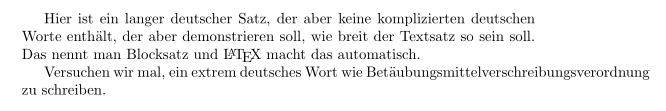
\includegraphics[width=.85\textwidth]{no_babel.png}
  \end{center}
  Mit \verb|\usepackage[ngerman]{babel}|:
  \begin{center}
    
\includegraphics[width=.85\textwidth]{babel.png}
  \end{center}
\end{frame}

\begin{frame}[fragile]{DIESE Tipps sorgen für mehr Struktur im \st{Leben} Dokument}
  Folgende Strukturelemente werden sehr häufig benötigt:
  \begin{center}
    \begin{tabular}{c>{\ttfamily}c}
      \toprule
      Element & Befehl \\
      \midrule
      Abschnitt & \textbackslash{}section\{ \emph{Name} \} \\
      Unterabschnitt & \textbackslash{}subsection\{ \emph{Name} \} \\
      Unter-Unterabschnitt & \textbackslash{}subsubsection\{ \emph{Name} \} \\
      Paragraph & \textbackslash{}paragraph\{ \emph{Name} \} \\
      \bottomrule
    \end{tabular}
  \end{center}
  Mag man keine Nummerierung, macht man das z.\,B.~so:
  \begin{center}
    \begin{verbatim}
      \section*{Sehr mysteriöse Überschrift}
    \end{verbatim}
  \end{center}
\end{frame}


\begin{frame}[fragile]{Strukturelemente}
  Aus den verwendeten Strukturelementen kann man sich ein Inhaltsverzeichnis
  via
  \begin{center}
    \begin{verbatim}
    \tableofcontents \end{verbatim}
  \end{center}
  generieren.
  Thematisch vielleicht nicht allzuweit entfernt:
  Titel können mit \verb|\maketitle| generiert werden.
  In der Preamble
  \begin{center}
    \begin{verbatim}
    \author{Ich\and Noch so einer}
    \date{today} % oder \date{04.~September~2021}
    \title{Ein Beitrag zu nutzloser Nischenwissenschaft
           mit unaussprechlichem Namen}
    \end{verbatim}
  \end{center}
\end{frame}

\begin{frame}[fragile]{Absätze}
  \begin{itemize}
    \item
      Whitespaces (also Leerzeichen und Tabs) sowie einfache
      Newline-Charaktere (\verb|\n|) werden als ein Leerzeichen gesehen.
    \item
      Will man einen Absatz machen (was man sehr oft sollte!), macht man das
      mit \emph{zwei} Newline-Charakteren bzw.~einer Leerzeile.
    \item
      Absätze sollten im Text \emph{NIE} mit \verb|\\| gesetzt werden.
    \item
      Normalerweise wird statt eines Absatzes ein Einzug gesetzt.
      Wer Absätze lieber mag, benutzt
  \end{itemize}
  \begin{center}
    \begin{verbatim}
    \setlength{\parindent}{0ex}
    \setlength{\parskip}{1ex plus 0.5ex minus 0.5ex}
    \end{verbatim}
  \end{center}
\end{frame}



\begin{frame}[fragile]{Seitenränder}
  Das \texttt{geometry}-Paket erlaubt eine extrem genaue Einstellung des
  Papierformats, z.\,B.~via
  \begin{center}
    \begin{verbatim}
    \usepackage[a4paper,
                left=3cm, right=3cm,
                top=2cm, bottom=2cm]{geometry}
    \end{verbatim}
  \end{center}
  Wesentlich einfacher zu bedienen ist
  \begin{center}
    \begin{verbatim}
    \usepackage[a4paper]{typearea}
    \end{verbatim}
  \end{center}
\end{frame}

\begin{frame}[fragile]{Formeln}
  \begin{itemize}
    \item
      Im Text ungefähr so: \verb|$a+b=c$|
    \item
      Zentriert (mit dem \texttt{amsmath}-Paket) mit
      \begin{center}
        \begin{verbatim}
        \begin{equation}
          \beta = 2.5\gamma
        \end{equation} \end{verbatim}
      \end{center}
    \item
      Mehrere Zeilen (mit Ausrichtung) so:
      \begin{center}
        \begin{verbatim}
        \begin{align}
          \beta  &= 2.5\cdot\gamma \\
          \alpha &= \frac{5}{\delta}.
        \end{align} \end{verbatim}
      \end{center}
    \item
      Nummerierung an- und ausschalten wieder mit dem Sternchen oder mit der
      \texttt{split}-Umgebung.
  \end{itemize}
\end{frame}

\begin{frame}[fragile]{Formeln die Zweite}
  \begin{itemize}
    \item \verb|\alpha \beta \gamma \rho \sigma \delta | gibt uns in
      einer Matheumgebung, also \verb|align| oder \verb|$...$|
      $\alpha \beta \gamma \rho \sigma \delta $.
    \item \verb|\times \otimes \oplus \cup \cap \cdot| gibt $\times \otimes
      \oplus \cup \cap \cdot$.
    \item \verb|< > \subset \supset \subseteq \supseteq \leq| und \verb|\geq| gibt
      \begin{equation}
        < > \subset \supset \subseteq \supseteq \leq \geq
      \end{equation}
    \item \verb|\int \oint \sum \prod| gibt $\int \oint \sum \prod$.
    \item \verb|F_{\text{rück}}| gibt $F_{\text{rück}}$, der Unterstrich gibt
      uns also ein Subskript und wir gehen in eine Text-Umgebung, weil der Text
      sonst kursiv wird ($Text\neq \text{Text} $).
    \item analog: \verb|F_{g} G_{\epsilon} h_{\epsilon\delta}| gibt $F_{g}
      G_{\epsilon} h_{\epsilon\delta}$.
  \end{itemize}
\end{frame}

\begin{frame}[fragile]{Formeln die Dritte}
  Normalerweise werden Whitespaces im Mathemodus vollständig ignoriert.
  Stattdessen darf man diese dann manuell setzen:
  \begin{center}
    \begin{tabular}{ccc}
      \verb|a\!b|      & gibt uns & $a\!b$, \\
      \verb|ab|        & gibt uns & $ab$, \\
      \verb|a\,b|      & gibt uns & $a\,b$, \\
      \verb|a\:b|      & gibt uns & $a\:b$, \\
      \verb|a\ b|      & gibt uns & $a\ b$, \\
      \verb|a\quad b|  & gibt uns & $a\quad b$, \\
      \verb|a\qquad b| & gibt uns & $a\qquad b$. \\
    \end{tabular}
  \end{center}
\end{frame}

\begin{frame}[fragile]{Formeln die Vierte (mit Integrieren und Ableiten!)}
  \begin{itemize}
    \item
      Integrale \verb|\int_{0}^{\infty} f(x)dx| macht
      \begin{equation*}
        \int_{0}^{\infty} f(x)dx.
      \end{equation*}
    \item
      \verb|\sum_{i=1}^{n} i^2 = \frac{n(n+1)(2n+1)}{6}| gibt
      \begin{equation*}
        \sum_{i=1}^n i^2 = \frac{n(n+1)(2n+1)}{6}.
      \end{equation*}
    \item
      \verb|\frac{\partial^2 f}{\partial x^2} (c)| gibt
      \begin{equation*}
        \frac{\partial^2 f}{\partial x^2}(c)
      \end{equation*}
  \end{itemize}
\end{frame}

\begin{frame}[fragile]{Dinge hervorheben}
	Manchmal möchte man ein \emph{Wort} im Satz betonen.
  Das geht mit \verb|\emph{Wort}|.
  Andere Fonts gibt's auch:
  \begin{center}
    \begin{tabular}{ccc}
      \toprule
      Befehl im Text & Befehl im Mathe-Modus & Beispiel \\
      \midrule
      \verb|\textbf{...}| & \verb|\mathbf{...}| & \textbf{Beispiel} \\
      \verb|\textrm{...}| & \verb|\mathrm{...}| & \textrm{Beispiel} \\
      \verb|\textsf{...}| & \verb|\mathsf{...}| & \textsf{Beispiel} \\
      \verb|\texttt{...}| & \verb|\mathtt{...}| & \texttt{Beispiel} \\
      \bottomrule
    \end{tabular}
  \end{center}
  Die sollte man im Text aber wenig bis gar nicht benutzen.
\end{frame}

\begin{frame}[fragile]{Bilder einfügen}
  Für Bilder benötigt:
  \begin{center}
    \verb|\usepackage{graphicx}|
  \end{center}
  Für Abbildungen braucht man eine \texttt{figure}-Umgebung.
  \begin{center}
    \begin{verbatim}
    \begin{figure}[htbp]
      \centering
      
\includegraphics[width=0.6\textwidth]{cat.png}
      \caption{Bild von einer Katze}%
      \label{fig:cat}
    \end{figure}
    \end{verbatim}
  \end{center}
\end{frame}

\begin{frame}[fragile]{Referenzen}
  Mit \verb|\label{|\emph{Name}\verb|}| kann man ein Label an alle möglichen
  Strukturelemente setzen.

  Verweise dann mit \verb|\ref{|\emph{Name}\verb|}| oder -- leicht
  intelligenter -- mit \verb|\cref{|\emph{Name}\verb|}|,
  benötigt
  \begin{center}
    \verb|\usepackage{cleveref}|
  \end{center}
  Nice and clicky:
  \begin{center}
    \verb|\usepackage{hyperref}|
  \end{center}
  (aber vor \verb|\usepackage{cleveref}|)
\end{frame}

\begin{frame}[fragile]{Tabellen}
  Tabellen selbst werden gesetzt in der (\texttt{table}- und)
  \texttt{tabular}-Umgebung.
  \begin{verbatim}
  \begin{table}[htbp]
    \centering
    \begin{tabular}{c|c|c|c}
      Wert 1 & Wert 2 & Wert 3 & Wert 4 \\ \hline
      1      & 35     & 12     & 15     \\
      32     & 12     & 33.5   & 1      \\
    \end{tabular}
    \caption{Unsere erste Tabelle}%
    \label{tab:erste_tabelle}
  \end{table} \end{verbatim}
  Anmerkung: \texttt{booktabs}-Paket für bessere Abstände.
\end{frame}

\begin{frame}[fragile]{Einheitenintermezzo}
  Das Formatieren von Zahlen und Einheiten ist manuell sehr nervig.
  Einfacher ist es mit \verb|\usepackage{siunitx}|.
  Wichtigste Befehle:
  \begin{center}
    \begin{tabular}{lc}
      \toprule
      \multicolumn{1}{c}{Befehl} & Ausgabe \\
      \midrule
      \verb|\SI{1.5 +- 0.3}{\joule\per\second\squared}|
      &
      \SI{1.5 +- 0.3}{\joule\per\second\squared}
      \\
      \verb|\si{\joule\per\second\squared}|
      &
      \si{\joule\per\second\squared}
      \\
      \verb|\num{2.4+-0.2e5}|
      &
      \num{2.4+-0.2e5}
      \\
      \bottomrule
    \end{tabular}
  \end{center}
\end{frame}

\begin{frame}[fragile]{Spaltentypenreferenz}
	\begin{center}
    \begin{tabular}{cp{5cm}}
      \toprule
      Buchstabe       & Spaltentyp \\
      \midrule
      \texttt{l}      & Links ausgerichtet \\
      \texttt{r}      & Rechts ausgerichtet \\
      \texttt{c}      & Zentriert \\
      \verb|p{2.5cm}| & Links ausgerichtet mit maximal \texttt{2.5cm} Breite \\
      \texttt{S}      & Spezieller \texttt{siunitx}-Typ \\
      \bottomrule
    \end{tabular}
  \end{center}
\end{frame}

\begin{frame}[fragile]{Hübschere Tabellen mit \texttt{siunitx}}
  \begin{center}
    \begin{verbatim}
    \begin{tabular}{%
      S[table-format=3.2(1)]
        ...
      }
      ...
    \end{tabular} \end{verbatim}
  \end{center}
  Das reserviert Platz für
  \begin{itemize}
    \item
      \texttt{3} Stellen vor dem Komma
    \item
      \texttt{2} Stellen nach dem Komma
    \item
      \texttt{1} zusätzliche Stelle für die Unsicherheit
  \end{itemize}
  Wichtig: Text muss in \verb|{...}| eingeschlossen werden!
\end{frame}

\begin{frame}[fragile]{Dateimanagement}
	Um größere Dokumente zu strukturieren, sollte man die Dateien aufspalten
  \begin{itemize}
    \item
      \verb|\input{filename}|:
      Einlesen des Inhalts der Datei \texttt{filename.tex}
    \item
      \verb|\include{filename}|:
      Einlesen der Datei \texttt{filename.tex} mit \verb|\clearpage| und so.
      Das kann benutzt werden, um sauber zwischen Abschnitten zu trennen. 
      Das ist schneller und kann mit \verb|\includeonly{filename}| in der
      Präambel kombiniert werden.
  \end{itemize}
\end{frame}

\begin{frame}[fragile]{Referenzmanagement}
  Am Ende eines Protokolls könnte (oder sollte!) eine Referenz-Liste
  existieren.
  Manuell geht das zum Beispiel so
  \begin{center}
    \begin{verbatim}
    \begin{thebibliography}{Kn1987}
      \bibitem[Kn86]{Knuth1986}
        Donald E.~Knuth. \emph{The TeXbook.} Addison-Wesley,1986
      \bibitem[Kn1987]{Knuth1987}
        Zufällige bibliographische Information
    \end{thebibliography}
    \end{verbatim}
  \end{center}
\end{frame}

\begin{frame}[fragile]{Referenzmanagement die Zweite}
  Die manuelle Methode sehr mühsam und unflexibel; außerdem erfordert es
  Kenntnisse von Zitierstilen.
  Alternativ nutzt man das \texttt{biblatex}-Paket (\emph{nicht}
  \texttt{bibtex}) mit dem \texttt{biber}-Programm (das ist separat zu
  installieren).
  \begin{center}
    \begin{verbatim}
      \usepackage[backend=biber, style=alphabetic]{biblatex}
      \addbibresource{mist.bib} \end{verbatim}
  \end{center}
  Im Dokument: \verb|\cite[Kapitel 2]{Kn86}| und am Ende:
  \verb|\printbibliography|.
\end{frame}

\begin{frame}[fragile]{Referenzmanagement die Zweite}
  Inhalt von \texttt{mist.bib}:
  \begin{center}
    \begin{verbatim}
    @Book{                Knuth1986,
       title        = {The TeXbook},
       author       = {Knuth, Donald E.},
       year         = {1986},
       publisher    = {Addison-Wesley},
    } \end{verbatim}
  \end{center}
  Das Kompilieren erfordert hierbei auch, dass \texttt{biblatex} mittendrin
  aufgerufen wird!
\end{frame}

\begin{frame}{Weitere Resourcen}
  \begin{itemize}
    \item
      \TeX{} StackExchange -- \url{tex.stackexchange.com}
    \item
      De\TeX ify -- \url{detexify.kirelabs.org/classify.html}
    \item
      texdoc -- entweder als Paket oder \url{texdoc.org/index.html}
  \end{itemize}
\end{frame}

\end{document}
